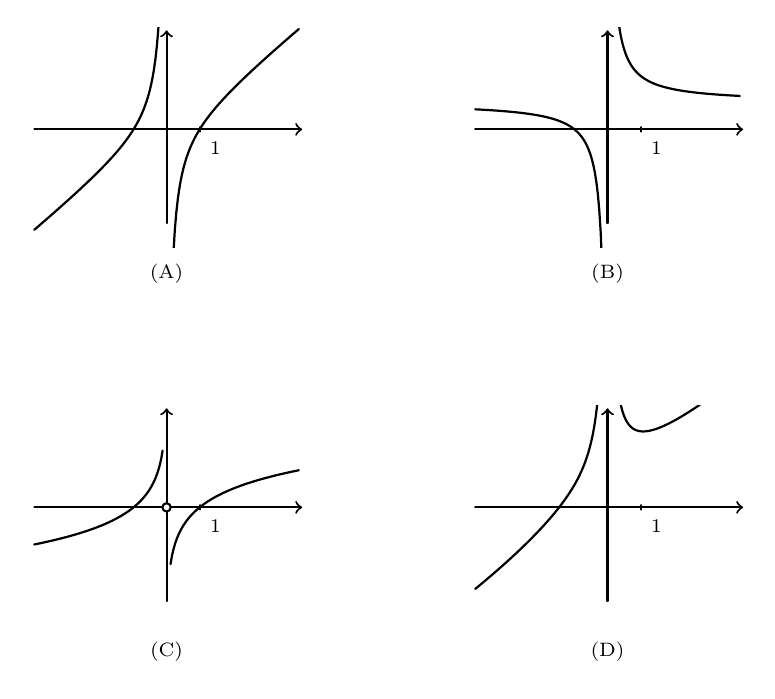
\begin{tikzpicture}[line cap=round,line join=round,line width=0.75pt,font=\scriptsize]
\begin{scope}[shift={(0,4.8)},x=0.42cm,y=0.34cm]
  \begin{scope}
  \clip (-4.2,-4.4) rectangle (4.2,3.8);
  \draw[->] (-4,0)--(4.1,0) node[right] {$x$};
  \draw[->] (0,-3.5)--(0,3.7) node[above] {$y$};
  \draw (1,0.08)--(1,-0.08) node[below right] {$1$};
  \draw[thick,domain=-4:-0.12,samples=90] plot (\x,{\x-1/\x});
  \draw[thick,domain=0.12:4,samples=90] plot (\x,{\x-1/\x});
  \end{scope}
  \node at (0,-5.4) {(A)};
\end{scope}
\begin{scope}[shift={(5.6,4.8)},x=0.42cm,y=0.34cm]
  \begin{scope}
  \clip (-4.2,-4.4) rectangle (4.2,3.8);
  \draw[->] (-4,0)--(4.1,0) node[right] {$x$};
  \draw[->] (0,-3.5)--(0,3.7) node[above] {$y$};
  \draw (1,0.08)--(1,-0.08) node[below right] {$1$};
  \draw[thick,domain=-4:-0.12,samples=90] plot (\x,{1+1/\x});
  \draw[thick,domain=0.12:4,samples=90] plot (\x,{1+1/\x});
  \end{scope}
  \node at (0,-5.4) {(B)};
\end{scope}
\begin{scope}[shift={(0,0)},x=0.42cm,y=0.34cm]
  \begin{scope}
  \clip (-4.2,-4.4) rectangle (4.2,3.8);
  \draw[->] (-4,0)--(4.1,0) node[right] {$x$};
  \draw[->] (0,-3.5)--(0,3.7) node[above] {$y$};
  \draw (1,0.08)--(1,-0.08) node[below right] {$1$};
  \draw[thick,domain=-4:-0.12,samples=90] plot (\x,{-ln(-\x)});
  \draw[thick,domain=0.12:4,samples=90] plot (\x,{ln(\x)});
  \filldraw[fill=white] (0,0) circle (1.5pt);
  \end{scope}
  \node at (0,-5.4) {(C)};
\end{scope}
\begin{scope}[shift={(5.6,0)},x=0.42cm,y=0.34cm]
  \begin{scope}
  \clip (-4.2,-4.4) rectangle (4.2,3.8);
  \draw[->] (-4,0)--(4.1,0) node[right] {$x$};
  \draw[->] (0,-3.5)--(0,3.7) node[above] {$y$};
  \draw (1,0.08)--(1,-0.08) node[below right] {$1$};
  \draw[thick,domain=-4:-0.12,samples=120] plot (\x,{1+\x+sin(deg(\x))/(\x^2)});
  \draw[thick,domain=0.12:4,samples=120] plot (\x,{1+\x+sin(deg(\x))/(\x^2)});
  \end{scope}
  \node at (0,-5.4) {(D)};
\end{scope}
\end{tikzpicture}
